\documentclass[a4paper,UTF8,titlepage]{ctexart}
\CTEXsetup[format={\Large\bfseries}]{section}
\usepackage{amsmath}
\usepackage{caption}
\usepackage{graphicx}
\usepackage{float}
%\usepackage{epsfig}
%\usepackage{subfig}
\usepackage{subfigure}
%\usepackage{subcaption}
\usepackage{diagbox}
\def\pgfsysdriver{pgfsys-dvipdfmx.def}
\usepackage{tikz}
\usepackage{hyperref}
\usepackage{amsfonts,amssymb}
\usepackage{blindtext}
\usepackage[T1]{fontenc}
\usepackage[utf8]{inputenc}
\usepackage{listings}
\pagestyle{plain}

% 用来设置附录中代码的样式

\lstset{
	basicstyle          =   \sffamily,          % 基本代码风格
	keywordstyle        =   \bfseries,          % 关键字风格
	commentstyle        =   \rmfamily\itshape,  % 注释的风格,斜体
	stringstyle         =   \ttfamily,  % 字符串风格
	flexiblecolumns,                % 别问为什么,加上这个
	numbers             =   left,   % 行号的位置在左边
	showspaces          =   false,  % 是否显示空格,显示了有点乱,所以不现实了
	numberstyle         =   \zihao{-5}\ttfamily,    % 行号的样式,小五号,tt等宽字体
	showstringspaces    =   false,
	captionpos          =   t,      % 这段代码的名字所呈现的位置,t指的是top上面
	frame               =   lrtb,   % 显示边框
}

\lstdefinestyle{Python}{
	language        =   Python, % 语言选Python
	basicstyle      =   \zihao{-5}\ttfamily,
	numberstyle     =   \zihao{-5}\ttfamily,
	keywordstyle    =   \color{blue},
	keywordstyle    =   [2] \color{teal},
	stringstyle     =   \color{magenta},
	commentstyle    =   \color{red}\ttfamily,
	breaklines      =   true,   % 自动换行,建议不要写太长的行
	columns         =   fixed,  % 如果不加这一句,字间距就不固定,很丑,必须加
	basewidth       =   0.5em,
}

\hypersetup{colorlinks=true,linkcolor=black}
\begin{document}
\title{带间断系数的弹性问题}
\date{\today}
\maketitle

\renewcommand{\abstractname}{\vspace{-2em}\large\bf 摘要}
\begin{abstract}
	
	客观世界下的很多能接触到的材料都不仅仅是单一的材料构成,往往由不同种材料复合而来。其中不同材料复合而来的物理现象所构成的数学模型即为界面问题。材料之间的间断面称之为界面, 且在上述模型中, 模型的解通常受间断系数的影响需要满足某种跳跃条件, 即服从某种意义上的守恒律. 界面问题在足够光滑的界面条件下,其解也会在此区域上光滑. 但是由于解在界面上的跳跃, 导致使用一般的数值解法很难在解的整体光滑性较差的情况下还能有比较理想的逼近效果和逼近精度.本文采用非协调有限元对二维情况下带间断系数的弹性问题进行求解  \\
	
	\noindent{\quad \quad \textbf{关键字:} 平面弹性问题; 间断系数;非协调有限元; locking-free}
\end{abstract}
\thispagestyle{empty}

\newpage

\renewcommand{\abstractname}{\vspace{-2em}\large\bf Abstract}
\begin{abstract}
	
	Many materials in the objective world that can be touched are not composed of a single material, but often composed of different materials. The mathematical model composed of the physical phenomena of different materials is called the interface problem. The discontinuous surface between materials is called the interface, and in the above model, the solution of the model usually needs to satisfy a certain jump condition under the influence of the discontinuous coefficient, that is, it obeys a certain sense of conservation law. The solution of the interface problem will also be smooth in this area under sufficiently smooth interface conditions. But because of the jump of the solution on the interface, it is difficult to use general numerical methods to achieve ideal approximation effect and approximation accuracy when the overall smoothness of the solution is poor. In this paper, nonconforming finite element method is used to solve the elastic problem with discontinuous coefficient in two-dimensional case.  \\
	
	\noindent{\quad \quad \textbf{Key words:} linear elasticity problem; discontinuous coefficient;nonconforming finite element; locking-free}
\end{abstract}
\thispagestyle{empty}

\newpage

\tableofcontents

\newpage

\section{绪论}

\subsection{研究背景}

具有间断系数的方程成为交界面问题。这类问题起源于许多应用领域,例如2种不同材料或者相同材料在不同状态下物理机制的研究 \textsuperscript{\cite{邵文婷2017求解一类交界面问题的模态基函数谱元法数值实验}}、声音在水中的传递、海市蜃楼现象等,同时在数值模拟等场景中也有者大量的界面问题。

平面弹性力学方程组是弹性力学中最基础、最常见的模型。当研究的弹性体形状和受力具有一定特点时,通过适当的简化处理,就可以归结为平面弹性问题 \textsuperscript{\cite{王兆清2018不可压缩平面问题的位移}}。
对于各向同性均匀介质的平面弹性问题,当材料的Lam$\acute{e}$常数$\lambda \to \infty$时,即对于几乎不可压介质,通常低阶的协调有限元解,往往不再收敛到原问题的解,或者达不到最优收敛阶,这就是闭锁现象\textsuperscript{\cite{陈绍春2007平面弹性的一个新的}}。

为了消除(近)不可压缩弹性问题中遇到的锁定现象,国内外研究学者提出了多种有效的数值分析方法。根据型函数建立过程中是否需要网格剖分,这些数值方法可以分为两类:一类是有网格方法,这其中包括
高阶有限元法\textsuperscript{\cite{peet2014legendre}}、
混合有限元法\textsuperscript{\cite{masud2011variational}}、
增强有限元法\textsuperscript{\cite{auricchio2005analysis}}和
不连续Galerkin法\textsuperscript{\cite{hansbo2003discontinuous}}等;
另一类是无网格方法,无网格方法又可分为弱形式无网格法和强形式的无网格方法\textsuperscript{\cite{王兆清2018不可压缩平面问题的位移}}。

本文将通过数值实验的方法,考察对于具有间断系数的平面弹性问题,使用C-R元是否仍可以解除闭锁现象。

\subsection{国内外研究现状}

1943年,R.W.Courant首次提出有限元法的核心思想。1956年,R.W.Clough等四位教授与工程师在科技期刊上发表一篇计算飞机机翼强度的论文,且把这种解法称之为刚性法(Stiffness),是有限元法在工程学界上的开端。1960年,R.W.Clough教授发表的平面弹性论文中,“有限元法”这个名称被首次使用,同时也将有限元法扩展到土木工程上。1963年,Richard MacNeal博士与Robert Schwendler联手创办了MSC公司,并开发了第一个软件程序,名为SADSAM,即数字仿真模拟结构分析,标志着有限元方法(FEA)由理论向程序的转变,1964-1965年,O.C.Zienkiewicz等人发表关于利用极小位能原理和虚功原理,以新的思路推导出有限元法。

我国有限元发展之路中较为著名的有:冯康(有限单元法理论),钱令希(余能定理),钱伟长(广义变分原理)等等。但是受限与当时的国际和国内环境,我国的学者在有限元方法上的进一步研究困难重重,很难跟上国际潮流,遗憾的被国外拉开距离。在之后的十年,伴随者国内有限元软件和有限元方法理论的诞生和发展,大型工程也逐渐使用有限元方法来计算,如水利、机械等多个领域,并且也都取得了不错的效果。上世纪90年代,国外的有限元软件大批量地涌入国内市场,涉及到各个领域。国外的学者专家也都进入各大学、工厂与企业进行宣传他们所掌握的技术和使用技巧,导致国内有限元发展更加困难。管理部门对有限元软件的认知上产生了偏差,对此失去了必要的支持,核心技术掌握在国外,所以至上世纪最后十几年里,国内自主技术创新的进度十分缓慢。但是进入21世纪后,国内自主知识产权的软件逐渐市场化,获得了一定的发展,同时也获得了国家对有限元技术的关注,逐渐走出低迷状态,有限元技术也不再仅仅停留在高校和企业中。

\section{有限元理论}

\subsection{Sobolev空间}

假定 G 是有界平面区域,其边界 $\Gamma$ 是按段光滑的简单闭曲线,$\overline{G} = G \cup \Gamma$ 是 G 的闭包。对于 $\overline{G}$ 上的任一函数 u(x,y),称集合{(x,y) | u(x,y) $\ne$ 0, (x,y) $\in \overline{G}$} 的闭包为 u 的支集。如果 u 的支集 $\in$ G 内,则说 u 于 G 具有紧致支集。具有紧致支集的函数必在边界 $\Gamma$ 的某一邻域内恒等于零\textsuperscript{\cite{李荣华2007偏微分方程数值解}}。

用 $C_0^{\infty} $ 表示 G 上无穷次可微并具有紧致支集的函数类,$L^2(G)$ 是定义在 G 上平方可积的可测函数空间,其内积和范数分别为

\begin{equation}
	(f,g) = \int_G fg dxdy
\end{equation}
\begin{equation}
	||f || = \sqrt{(f,f)} = (\int_G |f|^2 dxdy)^{\frac{1}{2}}
\end{equation}

对 $f \in L^2(G)$,如果存在g,h $\in L^2(G)$,使等式

\begin{equation}
	\int_G g \varphi dxdy = - \int_g f \frac{\partial \varphi}{\partial x} dxdy 
\end{equation}
\begin{equation}
	\int_G h \varphi dxdy = - \int_G f \frac{\partial \varphi}{\partial y} dxdy
\end{equation}

对任意的 $\varphi \in C_0^{\infty}$ 成立,则说 f 对 x 的一阶广义导数 g 和对 y 的一阶导数 h,记作

\begin{equation}
	f_x = \frac{\partial f}{\partial x} = g
\end{equation}
\begin{equation}
	f_y = \frac{\partial f}{\partial y} = y
\end{equation}

定义 
$$
	H^1(G) = \{f(x,y) | f, f_x, f_y \in L^2(G) \}
$$
其中 $f_x, f_y $ 是 f 的广义导数。与 $H^1(G)$ 引入内积
\begin{equation}
	(f,g)_1 = \int_G [fg + f_x g_x + f_y g_y] dxdy
\end{equation}
和范数
\begin{equation}
	||f||_1 = \sqrt{(f,f)} = (\int_G [|f|^2 + |f_x|^2 + |f_y|^2] dxdy )^{\frac{1}{2}}
\end{equation}

则 $H^1$ 是 Hilbert 空间,称之为 Sobolev 空间。

\subsection{弹性问题}

\subsubsection{边值问题}

令$u$,$g$,$t$,$\sigma=(\sigma_{ij})_{1 \le i,j \le 2}$, $\tau = (\tau_{ij})_{1\le i,j \le 2}$ 是双变量函数,定义以下符号
$$
\begin{matrix}
	\epsilon(u) = \frac{1}{2} (grad u + (grad u)^t) \\
	tr(\tau) = \tau_{11} + \tau_{22} \\
	grad(u) = \begin{pmatrix}
		\frac{\partial u_1}{\partial x} & \frac{\partial u_1}{\partial y} \\
		\frac{\partial u_2}{\partial x} &
		\frac{\partial u_2}{\partial y}
	\end{pmatrix} \\
	\delta = \begin{pmatrix}
		1 & 0 \\
		0 & 1
	\end{pmatrix} \\
	div u = \frac{\partial u_1}{\partial x} + \frac{\partial u_2}{\partial y} \\
	div \tau = \begin{pmatrix}
		\frac{\partial \tau_{11}}{\partial x} + \frac{\partial \tau_{12}}{\partial y} \\
		\frac{\partial \tau_{12}}{\partial x} + \frac{\partial \tau_{22}}{\partial 
			y} 
	\end{pmatrix} \\
	\sigma : \tau = \sum\limits_{i=1}^{2} \sum\limits_{j=1}^{2} \sigma_{ij} \tau_{ij}
\end{matrix}
$$

考虑各项同性弹性材料,令u(x,y),f(x,y)是其位移和体力,由线弹性问题的静态理论,u,f满足以下方程

\begin{equation}
\begin{aligned}
	-div \sigma(u) = f \quad  \in \Omega 
	%(\sigma(u) \nu) |_{\Gamma2} = t
\end{aligned}
\label{elasiticityEq}
\end{equation}

应力张量 $\sigma(u)$ 定义为
\begin{equation}
\sigma(u) = 2 \mu \epsilon(u) + \lambda tr(\epsilon(u)) \delta
\end{equation}

其中 $\Omega \in \mathbb{R}^2$,正常数$\lambda$, $\mu$为 Lam$\acute{e}$ 常数。假定$(\mu, \lambda) \in [\mu_1,\mu_2] \times (0, +\infty)$。

令 $\Gamma_1$、$\Gamma_2$ 为 $\partial \Omega$ 的两个开子集,使得 $\partial \Omega = \overline{\Gamma_1} \bigcup \overline{\Gamma_2}$ 并且 $\overline{\Gamma_1} \bigcap \overline{\Gamma_2} = \emptyset$,令$\Gamma_1$上的位移边界条件为
\begin{equation}
	u|_{\Gamma_1} = g
\end{equation}
并且$\Gamma_2$上的牵引力边值条件为
\begin{equation}
	(\sigma(u) \nu) |_{\Gamma_2} = t
\end{equation}

如果$\Gamma_1 = \emptyset$ (或 $\Gamma_2 = \emptyset$),则边值问题为纯牵引力(或纯位移)问题。

\subsubsection{变分}

对于齐次纯位移问题,令u在边界上满足
\begin{equation}
u |_{\partial \Omega} = 0
\label{qcbjtj}
\end{equation}

设 $\nu = (\nu_1,\nu_2)^t, \quad \nu_1, \nu_2 \in C_0^{\infty}(\Omega)$,方程 $\eqref{elasiticityEq}$ 两边同乘 $\nu$ 并积分得

\begin{equation}
-\int_{\Omega} div \sigma(u) \nu dxdy = \int_{\Omega} f \nu dxdy
\label{dycjf}
\end{equation}

参考文献知\textsuperscript{\cite{陈纪修2004数学分析}}

\begin{equation}
	f div a = div(fa) - a : grad f 
\label{fbjf}
\end{equation}
\begin{equation}
	\int_{\Omega} div a dV = \int_{\partial \Omega} a dS
\label{sddl}
\end{equation}

将边界条件$\eqref{qcbjtj}$,方程$\eqref{fbjf}$,$\eqref{sddl}$带入方程$\eqref{dycjf}$得

\par \quad \quad
$-\int_{\Omega} div \sigma(u) \nu dxdy$
$$ 
\quad \quad
\begin{matrix}
	\begin{aligned}
		&= -\int_{\Omega} div(\sigma(u) \nu) dxdy - \int_{\Omega} \sigma(u) : grad \nu dxdy \\
		&= -\int_{\Gamma} \sigma(u) \nu dxdy + \int_{\Omega} \sigma(u) : grad \nu dxdy \\
		&= \int_{\Omega} \sigma(u) : grad \nu dxdy \\
		&= \int_{\Omega} 2 \mu \epsilon(u) : grad \nu + \lambda div u div \nu dxdy  \\
		&= \mu \int_{\Omega} grad u : grad \nu dxdy + (\mu +\lambda) \int_{\Omega} div u div \nu  dxdy
	\end{aligned}
\end{matrix}
$$

所以

\begin{equation}
\mu \int_{\Omega} grad u : grad \nu dxdy + (\mu +\lambda) \int_{\Omega} div u div \nu  dxdy = \int_{\Omega} f \nu dxdy
\end{equation}

\textbf{该问题的变分问题为},求$u \in H^1(\Omega)$ 使得 $u |_{\Gamma_1} = 0$,并且
\begin{equation}
a(u,\nu) = \int_{\Omega} f \cdot \nu dxdy \quad \forall \nu \in V
\label{bffc}
\end{equation}
\par
其中

\begin{equation}
	\begin{aligned}
		a(u,\nu) :&= \mu \int_{\Omega} grad u : grad \nu dxdy + (\mu +\lambda) \int_{\Omega} div u div \nu  dxdy \\  		
		V :&= \{ \nu \in H^1(\Omega) \quad | \quad \nu |_{\Gamma} = 0 \}
	\end{aligned}
\end{equation}

\textbf{Lax-Milgram定理\textsuperscript{\cite{brenner2008mathematical}}:} 设 H 是 Hilbert 空间,$a(\bullet,\bullet)$ 是 $H \times H$ 上的有界的强制的双线性泛函。则对任意的$F \in H$,存在唯一的 $u \in H$ 满足
\begin{equation}
	a(u,\nu) = (f,\nu), \quad \forall \nu \in H 
\end{equation}

由Lax-Milgram定理知,此变分问题的解存在且唯一。

%证其与原问题的等价性

%\begin{enumerate}
%	\item 若 u 为原问题的解 \\


%	\item 若 u 为变分问题的解 \\
%	由
%	\par \quad \quad
%	$\int_{\Omega} \sigma(u) : grad \nu dxdy$
%	$$
%	\quad \quad
%	\begin{matrix}
	%		\begin{aligned}
		%			&= -\int_{\Gamma} \sigma(u) \nu dxdy + \int_{\Omega} \sigma(u) : grad %\nu dxdy \\
		%			&= -\int_{\Omega} div \sigma(u) \nu dxdy
		%		\end{aligned}
	%	\end{matrix} 
%	$$
%
%	得
%	$$
%		-\int_{\Omega} div \sigma(u) \nu dxdy = \int_{\Omega} f \nu dxdy
%	$$
%	
%	由变分法基本引理得
%	$$
%		-div \sigma(u) = f
%	$$
%	
%\end{enumerate}

\subsubsection{引入间断系数}

设 $\Omega_1$,$\Omega_2$ 是 $\Omega$ 的两个子集,使得 $\Omega_1 \bigcup \Omega_2 = \Omega$ 并且 $\Omega_1 \bigcap \Omega_2 = \emptyset$,

考虑以下边值问题
\begin{equation}
\begin{aligned}
	-div \sigma(u) &= f \quad \in \Omega \\
	u |_{\partial \Omega} &= 0
\end{aligned}
\end{equation}

当Lam$\acute{e}$ 常数 $\lambda$,$\mu$ 在 $\Omega_1$,$\Omega_2$ 上取不同值,即 $(x,y) \in \Omega_1$ 时 $\lambda = \lambda_1$,$\mu = \mu_1$,$(x,y) \in \Omega_2$ 时 $\lambda = \lambda_2$,$\mu = \mu_2$,$\lambda_1 \ne \lambda_2$,$\mu_1 \ne \mu_2$,通过计算得到与此问题对应的双线性形式为
\begin{equation}
\begin{aligned}
	a(u,\nu) &= \mu_1 \int_{\Omega_1} grad u : grad \nu dxdy + (\mu_1 +\lambda_1) \int_{\Omega_1} div u div \nu  dxdy \\
	&+ \mu_2 \int_{\Omega_2} grad u : grad \nu dxdy + (\mu_2 +\lambda_2) \int_{\Omega_2} div u div \nu  dxdy
\end{aligned}
\end{equation}

\subsection{离散}

\subsubsection{Galerkin法}

\begin{figure}[h]
	\centering
	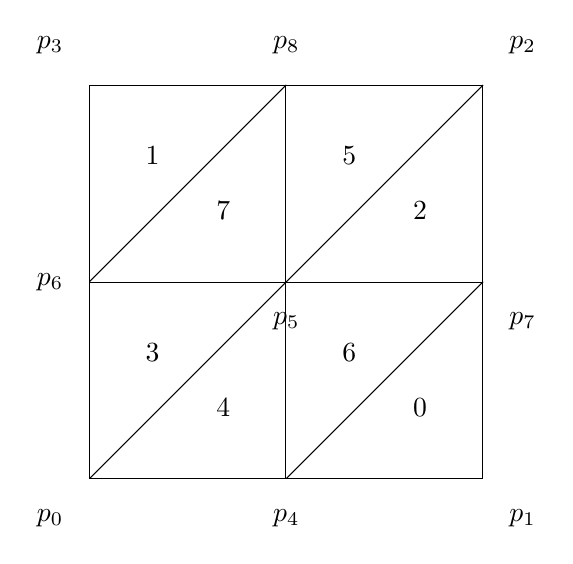
\begin{tikzpicture}
		\draw [step=71pt] (0,5) grid (5,0);
		
		\draw (0,0)--(5,5);
		\draw (0,2.5)--(2.5,5);
		\draw (2.5,0)--(5,2.5);
		
		\node at(-0.5,-0.5) {$p_0$};
		\node at(2.5,-0.5)  {$p_4$};
		\node at(5.5,-0.5)  {$p_1$};
		\node at(-0.5,2.5)  {$p_6$};
		\node at(2.5,2)     {$p_5$};
		\node at(5.5,2)     {$p_7$};
		\node at(-0.5,5.5)  {$p_3$};
		\node at(2.5,5.5)   {$p_8$};
		\node at(5.5,5.5)   {$p_2$};
		
		\node at(0.8,1.6) {3};
		\node at(1.7,0.9) {4};
		\node at(3.3,1.6) {6};
		\node at(4.2,0.9) {0};
		\node at(0.8,4.1) {1};
		\node at(1.7,3.4) {7};
		\node at(3.3,4.1) {5};
		\node at(4.2,3.4) {2};
	\end{tikzpicture}
	\caption{}
	\label{hf}
\end{figure}

设求解区间$\Omega = [0,1] \times [0,1]$,首先对其按照图$\ref{hf}$进行网格剖分,节点为
$$
p_0, p_1, ... , p_n 
$$
图中的三角形区域称为单元。

其次,在Sobolev空间 $H^1$ 内取子空间 $U_h$,它的元素在每一单元是次数不超过某一正整数 m 的多项式,在全区域 $\Omega$ 上属于函数空间 $H^1$。则 $U_h \times U_h$ 为试探函数空间。

设
$$
\begin{matrix}
	U_h = span(\varphi_0, \varphi_1, ... , \varphi_n) \\
	\phi_{2i} = (\varphi_i, 0), \quad \phi_{2i+1} = (0, \varphi_i), \quad i=0,...,n
\end{matrix}
$$

则 $\forall u_h \in U_h \times U_h$,可表成
\begin{equation}
	u_h = \sum\limits_{i=0}^{2n+1} c_i \phi_i
	\label{uh}
\end{equation}

将式 $\eqref{uh}$ 带入方程 $\eqref{bffc}$中得到 Galerkin 方程
\begin{equation}
	\sum\limits_{i=0}^{2n+1} a(\phi_i, \phi_j) c_i = (f,\phi_j), \quad j = 0, 1, ... , 2n+1 
	\label{galerkin}
\end{equation} 

令

$$
\begin{matrix}
	A = (a(\phi_j, \phi_i))_{0 \le i,j \le 2n+1} \\
	F = ((f,\phi_i))_{0 \le i \le 2n+1} \\
	c = (c_i)_{0 \le i \le 2n+1}
\end{matrix}
$$

则 Galerkin 方程$\eqref{galerkin}$的矩阵形式为

\begin{equation}
	Ac = F
\end{equation}

模型为齐次边界条件,若$(x_i,y_i)$为边界点,则 A 第 2i 行第 2i 列,第 2i+1 行第 2i+1 列元素为1,第 2i 和 2i+1 行的其他元素及  F(2i),F(2i+1) 都为0。

\subsubsection{线性元}

如图$\ref{xxy}$,设 $ \bigtriangleup(p_0,p_1,p_2) $ 是以 $p_0,p_1,p_2$ 为顶点的任意三角型元,面积为S。在 $ \bigtriangleup (p_0,p_1,p_2) $ 内任取一点p,坐标为$(x,y)$。过p点作与三个顶点的连线,将 $ \bigtriangleup(p_0,p_1,p_2) $ 分成三个三角形: $ \bigtriangleup(p_1,p_2,p), \bigtriangleup(p_0,p,p_2), \bigtriangleup(p_0,p_1,p) $,其面积分别为$S_0,S_1,S_2$ \textsuperscript{\cite{李荣华2007偏微分方程数值解}}

%\begin{figure}[hbt]
%	\centering
%\includegraphics[height=3cm,width=4cm]{../image/TriangleElement.png}
%	\caption{}
%	\label{SampleOfDatasets}
%\end{figure}

\begin{figure}[h]
	\centering
	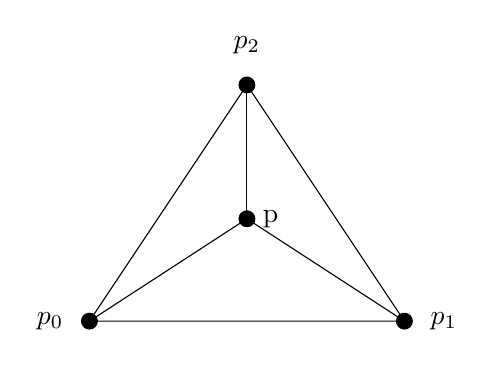
\begin{tikzpicture}
		\draw (3,0)--(7,0)--(5,3)--cycle;
		\draw (3,0)--(5,1.3)--(7,0);
		\draw (5,1.3)--(5,3);
		\filldraw (3,0)   circle(.1)
		(7,0) circle(.1)
		(5,3) circle(.1)
		(5,1.3) circle(.1);
		\node at(2.5,0)  {$p_0$};
		\node at(7.5,0)   {$p_1$};
		\node at(5,3.5)   {$p_2$};
		\node at(5.3,1.3) {p};
	\end{tikzpicture}
	\caption{}
	\label{xxy}
\end{figure}

显然$S_0 + S_1 + S_2 = S$,令
\begin{equation}
L_0 = \frac{S_0}{S}, \quad L_1 = \frac{S_1}{S}, \quad L_2 = \frac{S_2}{S}
\end{equation}
\par
%称$(L_0,L_1,L_2)$位$P_3$的面积坐标,其中
%$$
%	\begin{cases}
	%		2S = \left| \begin{matrix}
		%				1 & x_0 & y_0 \\
		%				1 & x_1 & y_1 \\
		%				1 & x_2 & y_2
		%			 \end{matrix} \right| ,
	%		 \quad
	%		 2S_0 = \left| \begin{matrix}
		%		 			1 & x   & y   \\
		%		 			1 & x_1 & y_1 \\
		%		 			1 & x_2 & y_2
		%		 \end{matrix} \right| 
	%		 \\
	%		2S_1 = \left| \begin{matrix}
		%					1 & x_0 & y_0 \\
		%					1 & x   & y   \\
		%					1 & x_2 & y_2
		%			   \end{matrix} \right|,
	%		\quad
	%		2S_2 = \left| \begin{matrix}
		%					1 & x_0 & y_0 \\
		%					1 & x_1 & y_1 \\
		%					1 & x   & y
		%			   \end{matrix} \right|
	%	\end{cases}
%$$

%由此可得面积坐标和直角坐标的转化关系
%$$
%\begin{cases}
%	x = x_0 L_0 + x_1 L_1 + x_2 L_2 \\
%	y = y_0 L_0 + y_1 L_1 + x_2 L_2
%\end{cases}
%$$
$$
\begin{cases}
	L_0 = \frac{1}{2S} [(x_2 y_3 - x_3 y_2) + (y_2 - y_3) x + (x_3 - x_2) y] \\
	L_1 = \frac{1}{2S} [(x_3 y_0 - x_0 y_3) + (y_3 - y_0) x + (x_0 - x_3) y] \\
	L_2 = \frac{1}{2S} [(x_0 y_1 - x_1 y_0) + (y_0 - y_1) x + (x_1 - x_0) y]
\end{cases} 
$$

因为

$$
\begin{cases}
	L_0 = \begin{cases}
		1, \quad x = x_0, y = y_0 \\
		0, \quad x = x_1, y = y_1 \\
		0, \quad x = x_2, y = y_2
	\end{cases} \\
	L_1 = \begin{cases}
		0, \quad x = x_0, y = y_0 \\
		1, \quad x = x_1, y = y_1 \\
		0, \quad x = x_2, y = y_2
	\end{cases} \\
	L_2 = \begin{cases}
		0, \quad x = x_0, y = y_0 \\
		0, \quad x = x_1, y = y_1 \\
		1, \quad x = x_2, y = y_2
	\end{cases} \\
\end{cases}
$$

所以在此区间上 $\varphi_i = L_i$,即

\begin{equation}
\begin{cases}
	\varphi_0 = \frac{1}{2S} [(x_2 y_3 - x_3 y_2) + (y_2 - y_3) x + (x_3 - x_2) y] \\
	\varphi_1 = \frac{1}{2S} [(x_3 y_0 - x_0 y_3) + (y_3 - y_0) x + (x_0 - x_3) y] \\
	\varphi_2 = \frac{1}{2S} [(x_0 y_1 - x_1 y_0) + (y_0 - y_1) x + (x_1 - x_0) y]
\end{cases} 
\end{equation}


\subsubsection{C-R元}

如图$\ref{CRElem}$,设三角形 $\bigtriangleup(q_0,q_1,q_2)$ 是以 $q0,q1,q2$ 为顶点的任意三角形元,$p_0,p_1,p_2$ 为其三条边的中点,其坐标分别为$(x_0.y_0),(x_1,y_1),(x_2,y_2)$。

\begin{figure}[h]
	\centering
	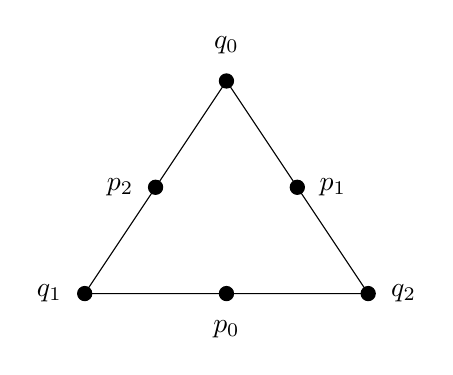
\begin{tikzpicture}[scale=0.9]
		\draw (0,0)--(4,0)--(2,3)--cycle;
		\filldraw (2,0)   circle(.1)
		(3,1.5) circle(.1)
		(1,1.5) circle(.1)
		(0,0) circle(.1)
		(4,0) circle(.1)
		(2,3) circle(.1);
		
		\node at(2,-0.5)  {$p_0$};
		\node at(3.5,1.5) {$p_1$};
		\node at(0.5,1.5) {$p_2$};
		
		\node at(-0.5,0) {$q_1$};
		\node at(4.5,0) {$q_2$};
		\node at(2,3.5) {$q_0$};
	\end{tikzpicture}
	\caption{}
	\label{CRElem}
\end{figure}

设三角形 $\bigtriangleup(q_0,q_1,q_2)$ 上的C-R元为 $\varphi_0, \varphi_1,\varphi_2$,

\begin{equation}
\varphi_i = a_i x + b_i y + c_i, \quad i = 0,1,2
\end{equation}

且其在 $p_0$,$p_1$,$p_2$ 点上满足以下关系式

\begin{equation}
\varphi_i(p_j) = \begin{cases}
	1, \quad i = j \\
	0, \quad i \ne j	
\end{cases}, \quad i, j = 0,1,2
\label{crjs}
\end{equation}

设

$$
A = \begin{bmatrix}
	x_0 & y_0 &1 \\
	x_1 & y_1 &1 \\
	x_2 & y_2 &1 \\
\end{bmatrix}, \quad 
c_i = (a_i,b_i,c_i)^t , \quad
f = (x,y,1)^t
$$

则方程组 $\eqref{crjs}$ 的矩阵形式为

\begin{equation}
A c_i = e_i, \quad i = 0,1,2
\end{equation}

通过计算可以得到单元$\bigtriangleup(q_0, q_1, q_2)$ 上的 C-R 元为

\begin{equation}
\varphi_i = A^{-1} e_i f, \quad i = 0,1,2
\end{equation} 

\iffalse
$$
\begin{cases}
	\begin{cases}
		\varphi_0(p_0) = a_0 x_0 + b_0 y_0 + c_0 = 1 \\
		\varphi_0(p_1) = a_0 x_1 + b_0 y_1 + c_0 = 0 \\
		\varphi_0(p_2) = a_0 x_2 + b_0 y_2 + c_0 = 0
	\end{cases} \\
	\begin{cases}
		\varphi_1(p_0) = a_1 x_0 + b_1 y_0 + c_1 = 0 \\
		\varphi_1(p_1) = a_1 x_1 + b_1 y_1 + c_1 = 1 \\
		\varphi_1(p_2) = a_1 x_2 + b_1 y_2 + c_1 = 0 
	\end{cases} \\
	\begin{cases}
		\varphi_2(p_0) = a_2 x_0 + b_2 y_0 + c_2 = 0 \\
		\varphi_2(p_1) = a_2 x_1 + b_2 y_1 + c_2 = 0 \\
		\varphi_2(p_2) = a_2 x_2 + b_2 y_2 + c_2 = 1
	\end{cases}
\end{cases}
$$
\fi

\subsection{误差估计}

假设$\Omega$是一个凸多边形区域,并且$\Gamma_1$ or $\Gamma_2$中任意一个为空。对于纯位移问题($\Gamma_2=\emptyset$),只考虑齐次边界条件。
\par
令$T^h$ 是$\Omega$ 三角划分的一个非退化族。对于纯位移问题($\Gamma_2=\emptyset$),我们使用有限元空间
% \begin{equation}\label{equ1} (\ref{newton})引用
	%	V_h := \{ \nu \in H^1(\Omega) : \nu |_{\emph{T}} \mbox{为线性函数}, \forall \emph{T} \in \emph{T}^h \}
	% \end{equation}
$$
V_h := \{ \nu \in H^1(\Omega) : \nu |_{T} , \forall T \in T^h \},
$$
并且对于纯牵引力问题($\Gamma_1 = \emptyset$),使用
% \begin{equation}\label{equ2}
	%	V_h :=
	%\end{equation}
	$$
	V_h := \{ \nu \in H^1(\Omega) : \nu |_{T} , \forall T \in T^h \},
	$$
%	\\ \\
%	根据第二章和第四章的理论我们得到以下定理。
	令 $u \in H^2(\Omega) \cap H^1(\Omega)$ 满足纯位移问题,并且$u_h \in V_h$ 满足
	\begin{equation}
	a(u_h, \nu) = \int_{\Omega} f \cdot \nu dx \quad \forall \nu \in V_h.
	\end{equation}
	\\
	则存在一个正常数$C_{(\mu, \lambda)}$ 使得\textsuperscript{\cite{brenner2008mathematical}}
	\begin{equation}
	\quad \quad \quad
	\| u - u_h \|_{H^1(\Omega)} \le C_{(\mu, \lambda)} h \| u \|_{H^2(\Omega)}.
	\end{equation}
	令 $u \in H^2(\Omega)$ 满足纯牵引力问题。令 $u_h \in V_h$ 满足
	\begin{equation}
	a(u_h,\nu) = \int_{\Omega} f \cdot \nu dx + \int_{\Gamma_2} t \cdot \nu ds \quad \forall \nu \in V_h.
	\end{equation}
	\\
	则存在一个正常数$C_{(\mu, \lambda)}$ 使得\textsuperscript{\cite{brenner2008mathematical}}
	\begin{equation}
	\| u - u_h \|_{H^1(\Omega)} \le C_{(\mu, \lambda)} h \| u \|_{H^2(\Omega)}.
	\end{equation}
%	对于一般情况 $ \emptyset \ne \Gamma_1 \ne \partial \Omega $ 下的收敛定理,查看练习 11.x.25. 
%	\\

\subsection{闭锁现象}

	对于固定的 $\mu$ 和 $\lambda$,以上定理给出了弹性问题令人满意近似的有限元近似。但是这些有限元方法的性能随着 $\lambda$ 趋向于 $\infty$ 而变差。这就是所谓的锁定现象\textsuperscript{\cite{brenner2008mathematical}}。
	\par 
	令 $\Omega = (0,1) \times (0,1)$. 考虑 $\mu = 1$ 时的纯位移边值问题:
	\begin{equation}
	\begin{aligned}
		div \{ 2 \epsilon (u^{\lambda}) + \lambda tr (\epsilon (u^{\lambda})) \delta \} &= f \quad in \quad \Omega \\ \quad \quad \quad \quad \quad 
		u^{\lambda}|_{\partial \Omega} &=  0.
	\end{aligned}
	\end{equation}
	注意给定的 f ,当 $\lambda \to \infty$,$\| div u^{\lambda} \|_{H^1(\Omega)} \to 0$.换句话说,我们正在处理一种几乎不可能压缩的弹性材料。为了强调对 $\lambda$ 的依赖,将应力张量 $\sigma_{\lambda}(\nu)$ 和 变分形式 $a_{\lambda}(\nu,\omega)$ 表示为
	\begin{equation}
	\begin{aligned}
		\sigma_{\lambda}(\nu) &= 2 \epsilon(\nu) + \lambda tr (\epsilon(\nu)) \delta \\
		a_{\lambda}(\nu,\omega) &= \int_{\Omega} \{ 2 \epsilon(\nu) : \epsilon(\omega) + \lambda div \nu div \omega \} dx.
	\end{aligned}
	\end{equation}
	
	令 $T^h$ 为 $\Omega $ (图$\ref{pf}$) 的一个规则三角剖分。对于每一个 $u \in H^2(\Omega) \cap H_0^1(\Omega)$,定义 $u_h^{\lambda} \in V_h$ 为以下方程组的特解
	\begin{equation}
	\begin{aligned}
		a_{\lambda}(u_h^{\lambda},\nu) &= \int_{\Omega} 
		[ -div \sigma_{\lambda}(u) ] \cdot \nu dx \quad \forall \nu \in V_h. \\
		V_h &:= \{ \nu \in H^1(\Omega) : \nu |_{T}, \forall T \in T^h \}
	\end{aligned}
	\end{equation}
	
%	\begin{figure}[hbt]
%		\centering
%		\includegraphics{../image/Fig.11.1.png}
%		\caption{单位正方形的规则三角剖分}
%	\end{figure}

\begin{figure}[ht]
	\centering
	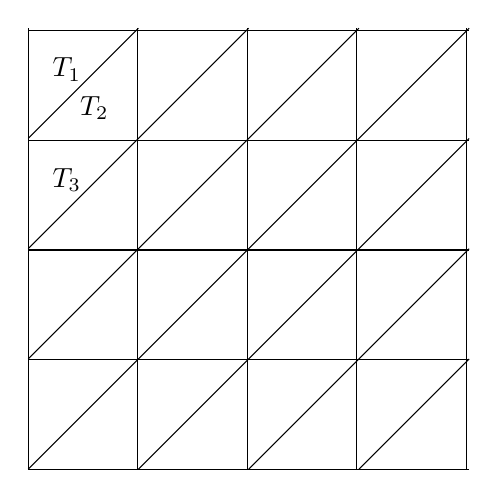
\begin{tikzpicture}[scale=0.7]
		\draw [step=56.56pt] (0,8) grid (8,0);
		
		\draw (0,6) -- (2,8);
		\draw (0,4) -- (4,8);
		\draw (0,2) -- (6,8);
		\draw (0,0) -- (8,8);
		\draw (2,0) -- (8,6);
		\draw (4,0) -- (8,4);
		\draw (6,0) -- (8,2); 
		
		\node at(0.7,7.25) {$T_1$};
		\node at(1.2,6.55) {$T_2$};
		\node at(0.7,5.25) {$T_3$};
	\end{tikzpicture}
	\caption{}
	\label{pf}
\end{figure}
	
	定义 $L_{\lambda,h}$ 为
	\begin{equation}
	L_{\lambda,h} := sup \{ \frac{|u-u_h^{\lambda}|_{H^1(\Omega)}}{\| div \sigma_{\lambda}(u) \|_{L^2(\Omega)}} : 0 \ne u \in H^2(\Omega) \cap H^1(\Omega) \}.
	\end{equation}
	\\ 
	则存在一个与 h 无关的正常数 C 使得\textsuperscript{\cite{brenner2008mathematical}}
	\begin{equation}
	\lim\limits_{\lambda \to \infty} \inf L_{\lambda,h} \ge C . \label{ab}
	\end{equation}
	式 $\eqref{ab}$ 意味着:无论 h 取多小,只要 $\lambda$ 足够大,我们都能找到 $u \in H^2(\Omega) \cap H^1(\Omega)$ 使得相对误差$ |u-u_h|_{H^1(\Omega)} / \| div \sigma_{\lambda}(u) \|_{L^2(\Omega)} $ 以一个与 h 无关的常数为下界。换句话说,有限元方法的性能将会随着 $\lambda$ 变大而变坏。
	\par
	\iffalse
	为证明式 $\eqref{ab}$,首先观察到
	$$
	\{ \nu \in V_h : div \nu = 0 \} = \{ 0 \}
	$$
	因此,映射 $\nu \to div \nu$ 是有限维空间 $V_h$ 到 $L^2(\Omega)$ 的一个一对一映射,并且存在一个正常数 $C_1(h)$ 使得
	$$
	\| \nu \|_{H^1(\Omega)} \le C_1(h) \| div \nu \|_{L^2(\Omega)} \quad \forall \nu \in V_h.
	$$
	令 $\psi$ 是 $\overline{\Omega}$ 上的无穷次可微函数,使得在 $\Omega$ 的边界上 $curl \psi = 0$ 且 $\| \epsilon(curl \psi) \|_{L^2(\Omega)} = 1$。令 $u := curl \psi$。则 $u \in H^2(\Omega) \cap H^1(\Omega)$,并有
	\begin{align}	
	div u = 0, \label{a2} \\
	\| \epsilon(u) \|_{L^2(\Omega)} = 1, \label{a3}\\
	\sigma_{\lambda}(u) = 2 \epsilon(u).  \label{a4}
	\end{align}
	根据 $\eqref{a2}$, $\eqref{a4}$ 和分步积分得
	\begin{align}
	- \int_{\Omega} div \epsilon(u) \cdot u dx = \int_{\Omega} \epsilon(u) : \epsilon(u) dx = 1. \label{a5}
	\end{align}
	根据 $\eqref{a4}$, $\eqref{a5}$ 推断
	$$
	\quad \quad \quad \quad \quad \quad \quad
	\lim\limits_{\lambda \to \infty} div \sigma_{\lambda}(u) = 2 div \epsilon(u) \ne 0. 
	$$
	由 (2.5.10) 得,
	$$
	a_{\lambda}(u-u_h^{\lambda}, u-u_h^{\lambda}) = \min\limits_{\nu \in V_h} a_{\lambda}(u-\nu,u-\nu) \le a_{\lambda}(u,u).
	$$
	由 $\eqref{a2}$ 和 $\eqref{a3}$,得到
	$$
	a_{\lambda}(u,u) = 2.
	$$
	因此,对于 $\lambda$ 足够大时有
	\begin{align} 
	a_{\lambda} (u-u_h^{\lambda}, u-u_h^{\lambda}) \le 2. \label{a6}
	\end{align}
	由 $\eqref{a2}$ 和 $\eqref{a6}$ 得
	\\
	$$
	\begin{matrix}
		\sqrt{\lambda} \| div u_h^{\lambda} \|_{L^2(\Omega)} = \sqrt{\lambda} \| div(u-u_h^{\lambda}) \|_{L^2(\Omega)} \\ 
		\quad \quad \quad \quad \quad \quad \quad
		\le \sqrt{a_{\lambda}(u-u_h^{\lambda}, u-u_h^{\lambda})} \\
		\le \sqrt{2}	
	\end{matrix}
	$$
	\\
	对足够大的 $\lambda$ 有
	$$
	\lim\limits_{\lambda \to \infty} \| div u_h^{\lambda} \|_{L^2(\Omega)} = 0.
	$$
	\\
	由式 $\eqref{ab}$ 有
	$$
	\lim\limits_{\lambda \to \infty} \| u_h^{\lambda} \|_{H^1(\Omega)} = 0.
	$$
	最后,得到 %(cf.exercise 11.x.16)
	$$ 
	\begin{matrix}
		\lim\limits_{\lambda \to \infty}\inf L_{\lambda,h} \ge \lim\limits_{\lambda \to \infty}\inf \frac{|u-u_h^{\lambda}|_{H^1(\Omega)}}{\| div \sigma_{\lambda}(u) \|_{L^2(\Omega)}} \\
		\quad \quad \quad \quad
		= \frac{|u|_{H^1(\Omega)}}{\| div \sigma(u) \|_{L^2(\Omega)}} > 0.
	\end{matrix}
	$$
	\fi

\section{算例}

\subsection{弹性问题}

\subsubsection{算例一}

考察以下边值问题
$$
\begin{matrix}
	-div \sigma(u) = f \quad \in \Omega  \\
	u |_{\partial \Omega} = 0
	%(\sigma(u) \nu) |_{\Gamma2} = t
\end{matrix}
$$ 
\par
其中$ u = (u_1,u_2)^t $ 为求解向量,$ f = (f_1,f_2)^t $为右端向量,$ \Omega = [0,1] \times [0,1] $
$$
\begin{matrix}
	u_1 = (x - 1)(y - 1) y sin(x) 
	\\
	u_2 = (x - 1)(y - 1) x sin(y) 
\end{matrix}
$$

通过数值实验得到,当 $\mu = \lambda = 1, 1E4, 1E8$ 时的误差及误差阶如下表

\begin{table}[h]
	\centering
	\caption{$|u-u_h|_{H^1(\Omega)}$}
	\scalebox{0.8}{
	\begin{tabular}{|c|c|c|c|c|c|c|} \hline
		\diagbox{$\lambda$}{h} &1.0 &0.5 &0.25 &0.125 &0.0625 &误差阶 \\ \hline
		1 &4.102804E-1 &1.424371E-1 &8.382384E-2 &4.737414-2 &2.528276E-2 &0.8305559 \\ \hline
		1E4 &4.102804E-1 &1.424371E-1 &8.382384E-2 &4.737414E-2 &2.528276E-2 &0.8305559  \\ \hline
		1E8 &4.102804E-1 &1.424371E-1 &8.382384E-2 &4.737414E-2 &2.528276E-2 &0.8305559 \\ \hline
	\end{tabular}}
\end{table}

数值解和精确解图像如下

\begin{figure}[ht]
	\centering
	\caption{}
	\subfigure[数值解图像]{
		\includegraphics[height=5.5cm,width=5.5cm]{../image/elaticity_uh_u/PDE1/uh_lam=1.png}
		\label{elsticity_uh_1}}	
	\subfigure[精确解图像]{
		\includegraphics[height=5.5cm,width=5.5cm]{../image/elaticity_uh_u/PDE1/u_lam=1.png}
		\label{elsticity_u_1}}
\end{figure}

\newpage

\subsubsection{算例二}

考察以下边值问题
$$
\begin{matrix}
	-div \sigma(u) = f \quad \in \Omega  \\
	u |_{\partial \Omega} = 0
	%(\sigma(u) \nu) |_{\Gamma2} = t
\end{matrix}
$$ 
\par
其中$ u = (u_1,u_2)^t $ 为求解向量,$ f = (f_1,f_2)^t $为右端向量,$ \Omega = [0,1] \times [0,1] $
$$
\begin{matrix}
	u_1 = x^2 sin(x-1) y^2 sin(y-1) 
	\\
	u_2 = x^2 sin(x-1) y^2 sin(y-1)
\end{matrix}
$$

通过数值实验得到,当 $\mu = \lambda = 1, 1E4, 1E8$ 时的误差及误差阶如下表

\begin{table}[h]
	\centering
	\caption{$|u-u_h|_{H^1(\Omega)}$}
	\scalebox{0.8}{
		\begin{tabular}{|c|c|c|c|c|c|c|} \hline
			\diagbox{$\lambda$}{h} &1.0 &0.5 &0.25 &0.125 &0.0625 &误差阶 \\ \hline
			1 &1.381670E-1 &1.038442E-1 &4.190134E-2 &2.135923E-2 &1.113314E-2 &1.063660 \\ \hline
			1E4 &1.381670E-1 &1.038442E-1 &4.190134E-2 &2.135923E-2 &1.113314E-2 &1.063660  \\ \hline
			1E8 &1.381670E-1 &1.038442E-1 &4.190134E-2 &2.135923E-2 &1.113314E-2 &1.063660 \\ \hline
	\end{tabular}}
\end{table}

数值解和精确解图像如下

\begin{figure}[ht]
	\centering
	\caption{}
	\subfigure[数值解图像]{
		\includegraphics[height=5.5cm,width=5.5cm]{../image/elaticity_uh_u/PDE2/uh_lam=1.png}
		\label{elsticity_uh_2}}	
	\subfigure[精确解图像]{
		\includegraphics[height=5.5cm,width=5.5cm]{../image/elaticity_uh_u/PDE2/u_lam=1.png}
		\label{elsticity_u_2}}
\end{figure}

\newpage

\subsubsection{算例三}

考察以下边值问题
$$
\begin{matrix}
	-div \sigma(u) = f \quad \in \Omega  \\
	u |_{\partial \Omega} = 0
	%(\sigma(u) \nu) |_{\Gamma2} = t
\end{matrix}
$$ 
\par
其中$ u = (u_1,u_2)^t $ 为求解向量,$ f = (f_1,f_2)^t $为右端向量,$ \Omega = [0,1] \times [0,1] $
$$
\begin{matrix}
	u_1 = -(x-1) (e^x-1) (y-1) (e^y-1)
	\\
	u_2 = -(x-1) (e^x-1) (y-1) (e^y-1) 
\end{matrix}
$$

通过数值实验得到,当 $\mu = \lambda = 1, 1E4, 1E8$ 时的误差及误差阶如下表

\begin{table}[ht]
	\centering
	\caption{$|u-u_h|_{H^1(\Omega)}$}
	\scalebox{0.8}{
		\begin{tabular}{|c|c|c|c|c|c|c|} \hline
			\diagbox{$\lambda$}{h} &1.0 &0.5 &0.25 &0.125 &0.0625 &误差阶 \\ \hline
			1 &8.170963E-1 &3.487612E-1 &1.669124E-1 &8.921846E-2 &4.718501E-2 &0.95611946 \\ \hline
			1E4 &8.170963E-1 &3.487612E-1 &1.669124E-1 &8.921846E-2 &4.718501E-2 &0.95611946  \\ \hline
			1E8 &8.170963E-1 &3.487612E-1 &1.669124E-1 &8.921846E-2 &4.718501E-2 &0.95611946 \\ \hline
	\end{tabular}}
\end{table}

数值解和精确解图像如下

\begin{figure}[h]
	\centering
	\caption{}
	\subfigure[数值解图像]{
		\includegraphics[height=5.5cm,width=5.5cm]{../image/elaticity_uh_u/PDE3/uh_lam=1.png}
		\label{elsticity_uh_3}}	
	\subfigure[精确解图像]{
		\includegraphics[height=5.5cm,width=5.5cm]{../image/elaticity_uh_u/PDE3/u_lam=1.png}
		\label{elsticity_u_3}}
\end{figure}

\newpage

\subsection{带间断系数的弹性问题}

\subsubsection{算例}

考察以下边值问题
$$
\begin{matrix}
	-div \sigma(u) = f \quad \in \Omega  \\
	u |_{\Gamma} = 0
	%(\sigma(u) \nu) |_{\Gamma2} = t
\end{matrix}
$$ 
\par
其中$ u = (u_1,u_2)^t $ 为求解向量,$ f = (f_1,f_2)^t $为右端向量,
$ 
\Omega = [0,1] \times [0,1] , \quad 
\Omega_1 = [0,0.5] \times [0,0.5] , \quad
\Omega_2 = [0.5,1] \times [0,0.5], \quad
\Omega_3 = [0,0.5] \times [0.5,1], \quad
\Omega_4 = [0.5,1] \times [0.5,1]
$ 
\par
当$(x,y) \in \Omega_1$时,$\mu = \lambda = \lambda_1$
$$
\begin{matrix}
	u_1 = x (x-0.5) (x-1) y (y-0.5) (y-1) / \lambda_1
	\\
	u_2 = x (x-0.5) (x-1) y (y-0.5) (y-1) / \lambda_1
\end{matrix}
$$

当$(x,y) \in \Omega_2$时, $\mu = \lambda = \lambda_2$

$$
\begin{matrix}
	u_1 = x (x-0.5) (x-1) y (y-0.5) (y-1) / \lambda_2 
	\\
	u_2 = x (x-0.5) (x-1) y (y-0.5) (y-1) / \lambda_2
\end{matrix}
$$

当$(x,y) \in \Omega_3$时,$\mu = \lambda = \lambda_3$
$$
\begin{matrix}
	u_1 = x (x-0.5) (x-1) y (y-0.5) (y-1) / \lambda_3
	\\
	u_2 = x (x-0.5) (x-1) y (y-0.5) (y-1) \ \lambda_3
\end{matrix}
$$

当$(x,y) \in \Omega_4$时, $\mu = \lambda = \lambda_4$

$$
\begin{matrix}
	u_1 = x (x-0.5) (x-1) y (y-0.5) (y-1) / \lambda_4 
	\\
	u_2 = x (x-0.5) (x-1) y (y-0.5) (y-1) / \lambda_4
\end{matrix}
$$
令 $\lambda = [\lambda_1, \lambda_2, \lambda_3, \lambda_4]$,$\mu = [\mu_1, \mu_2, \mu_3, \mu_4]$

\begin{enumerate} 
	
\newpage
	
\item 当 $\lambda = \mu= [1,2,3,4]$ 时误差如下

\begin{table}[h]
	\centering
	\caption{$|u-u_h|_{H^1(\Omega)}$}
	\scalebox{0.8}{
		\begin{tabular}{|c|c|c|c|c|c|} \hline
			h &0.5 &0.25 &0.125 &0.0625 &误差阶 \\ \hline
			$|u-u_h|_{H^1(\Omega)}$ &1.984010E-1 &8.447614E-1 &4.446847E-1 &2.373949E-2 &0.9156274 \\ \hline
	\end{tabular}}
\end{table}

\begin{figure}[h]
	\centering
	\caption{}
	\subfigure[数值解图像]{
		\includegraphics[height=5.5cm,width=5.5cm]{../image/interface_uh_u/uh_lam=[1. 2. 3. 4.].png}
		\label{interface_uh_0}}	
	\subfigure[精确解图像]{
		\includegraphics[height=5.5cm,width=5.5cm]{../image/interface_uh_u/uh_lam=[1. 2. 3. 4.].png}
		\label{interface_u_0}}
\end{figure}

\newpage

\item 当 $\lambda = \mu= [1E4,2E4,3E4,4E4]$ 时误差如下

\begin{table}[h]
	\centering
	\caption{$|u-u_h|_{H^1(\Omega)}$}
	\scalebox{0.8}{
		\begin{tabular}{|c|c|c|c|c|c|} \hline
			h &0.5 &0.25 &0.125 &0.0625 &误差阶 \\ \hline
			$|u-u_h|_{H^1(\Omega)}$ &1.984010E-1 &8.447614E-1 &4.446847E-1 &2.373949E-2 &0.9156274 \\ \hline
	\end{tabular}}
\end{table}

\begin{figure}[h]
	\centering
	\caption{}
	\subfigure[数值解图像]{
		\includegraphics[height=5.5cm,width=5.5cm]{../image/interface_uh_u/uh_lam=[1. 2. 3. 4.].png}
		\label{interface_uh_4}}	
	\subfigure[精确解图像]{
		\includegraphics[height=5.5cm,width=5.5cm]{../image/interface_uh_u/uh_lam=[1. 2. 3. 4.].png}
		\label{interface_u_4}}
\end{figure}

\newpage

\item 当 $\lambda = \mu= [1E8,2E8,3E8,4E8]$ 时误差如下

\begin{table}[h]
	\centering
	\caption{$|u-u_h|_{H^1(\Omega)}$}
	\scalebox{0.8}{
		\begin{tabular}{|c|c|c|c|c|c|} \hline
			h &0.5 &0.25 &0.125 &0.0625 &误差阶 \\ \hline
			$|u-u_h|_{H^1(\Omega)}$ &1.984010E-1 &8.447614E-1 &4.446847E-1 &2.373949E-2 &0.9156274 \\ \hline
	\end{tabular}}
\end{table}

\begin{figure}[h]
	\centering
	\caption{}
	\subfigure[数值解图像]{
		\includegraphics[height=5.5cm,width=5.5cm]{../image/interface_uh_u/uh_lam=[1. 2. 3. 4.].png}
		\label{interface_uh_8}}	
	\subfigure[精确解图像]{
		\includegraphics[height=5.5cm,width=5.5cm]{../image/interface_uh_u/uh_lam=[1. 2. 3. 4.].png}
		\label{interface_u_8}}
\end{figure}

\end{enumerate}

\section{总结}

本文使用 C-R 有限元方法求解了带间断系数的平面弹性问题,分析了非协调元对闭锁现象的影响。数值结果表明,当 Lam$\acute{e}$ 常数间断且相等时,C-R 元可以有效地解除闭锁现象,并且具有预期的收敛阶。

为了完善本文的研究,未来可以考虑对纯牵引力问题进行数值实验,以检验 C-R 元在不同的边界条件下的表现。同时,也可以通过改变间断系数的大小和形式,以及使用不同的网格划分方式,来进一步探究 C-R 元的有效性和稳定性,以及对间断系数的敏感性。

\newpage
\vfill

\CTEXsetup[format={\large\bfseries\songti\centering},beforeskip=0.5em,afterskip=0.5em]{section}
\bibliographystyle{unsrt}
\clearpage
\phantomsection
\addcontentsline{toc}{section}{参考文献}
\tolerance=500
\bibliography{interface_problem}

\newpage

%\chapter{\centerline{致谢}}
\section*{致谢}
\addcontentsline{toc}{section}{致谢}

时光荏苒, 岁月如梭, 转眼间大学生活来到了最后阶段. 当我写完这篇毕业论文的时候, 有一种如释重负的感觉, 感慨颇多. 回首大学四年, 得到过太多人的帮助了. 首先诚挚的感谢我的论文指导老师王华老师. 本文的研究工作都是在王华老师的悉心指导下完成的. 王老师平易近人, 严谨务实, 由于我知识储备不足, 在论文撰写过程中遇到了许多困难和疑惑, 王华老师都及时给予指点, 耐心解释所犯的错误, 投入了大量的心血和精力, 更是不厌其烦地帮我察看论文中的小漏洞. 王华老师对我的帮忙和关怀实在无法用言语表明. 还要感谢所有的老师们, 正是因为有了他们的督促和教导才能让我在这四年的学习生活里受益匪浅, 快速汲取专业知识, 提升专业能力. 同时也要感谢组内的同学们, 是他们以极大的热情来解答我在理论和程序上的疑问, 帮忙收集资料, 让平淡的日子不再那么枯燥乏味. 最后还要感谢我的家人, 是他们的支持与付出才给了我学习的机会, 感谢一直对我的理解, 这是我不断前进的动力. 

\newpage

\appendix
\section{附录 数值程序}

\lstinputlisting[
style       =   Python,
caption     =   {\bf elasticityCR.py},
label       =   {elasticityCR.py}
]{../program/toPdf/elasticityCR.py}

\lstinputlisting[
style       =   Python,
caption     =   {\bf tool.py},
label       =   {tool.py}
]{../program/toPdf/tool.py}

\end{document}